% !TEX TS-program = pdflatex
% !TEX encoding = UTF-8 Unicode

% This is a simple template for a LaTeX document using the "article" class.
% See "book", "report", "letter" for other types of document.

\documentclass[20pt]{article} % use larger type; default would be 10pt

\usepackage[utf8]{inputenc} % set input encoding (not needed with XeLaTeX)

%%% Examples of Article customizations
% These packages are optional, depending whether you want the features they provide.
% See the LaTeX Companion or other references for full information.

%%% PAGE DIMENSIONS
\usepackage{geometry} % to change the page dimensions
\geometry{a4paper} % or letterpaper (US) or a5paper or....
% \geometry{margin=2in} % for example, change the margins to 2 inches all round
% \geometry{landscape} % set up the page for landscape
%   read geometry.pdf for detailed page layout information

\usepackage{graphicx} % support the \includegraphics command and options

% \usepackage[parfill]{parskip} % Activate to begin paragraphs with an empty line rather than an indent

%%% PACKAGES
\usepackage{booktabs} % for much better looking tables
\usepackage{array} % for better arrays (eg matrices) in maths
\usepackage{paralist} % very flexible & customisable lists (eg. enumerate/itemize, etc.)
\usepackage{verbatim} % adds environment for commenting out blocks of text & for better verbatim
%\usepackage{subfig} % make it possible to include more than one captioned figure/table in a single float
\usepackage{mathtools}
\usepackage{graphicx} % supports images in latex
% These packages are all incorporated in the memoir class to one degree or another...

\usepackage{graphicx}
\usepackage{subcaption}

%%% Other stuff
\DeclarePairedDelimiter\ceil{\lceil}{\rceil}
\DeclarePairedDelimiter\floor{\lfloor}{\rfloor}

%%% HEADERS & FOOTERS
\usepackage{fancyhdr} % This should be set AFTER setting up the page geometry
\pagestyle{fancy} % options: empty , plain , fancy
\renewcommand{\headrulewidth}{0pt} % customise the layout...
\lhead{}\chead{}\rhead{}
\lfoot{}\cfoot{\thepage}\rfoot{}

%%% SECTION TITLE APPEARANCE
\usepackage{sectsty}
\allsectionsfont{\sffamily\mdseries\upshape} % (See the fntguide.pdf for font help)
% (This matches ConTeXt defaults)

%%% ToC (table of contents) APPEARANCE
\usepackage[nottoc,notlof,notlot]{tocbibind} % Put the bibliography in the ToC
\usepackage[titles,subfigure]{tocloft} % Alter the style of the Table of Contents
\renewcommand{\cftsecfont}{\rmfamily\mdseries\upshape}
\renewcommand{\cftsecpagefont}{\rmfamily\mdseries\upshape} % No bold!

%%% Code syntax highliting
\usepackage{listings}
%\begin{lstlisting}[language=java]
%\end{lstlisting}

%%% graphics path \graphicspath{{./HW5}}

%%% END Article customizations

%%% nice things to keep around

% \noindent\rule{2cm}{0.4pt} 
%%% puts a small horizontal line

% \mathcal{O} 
%%% big O notation

%\begin{figure}[!htbp]
%  	\centering
%   	\begin{subfigure}[p]{0.5\linewidth}
%    	\includegraphics[width=\linewidth]{}
%   	\end{subfigure}
%\end{figure} 

%%% The "real" document content comes below...

\title{Computational Statistics Homework 1}
\author{Liam Dillingham}
%\date{} % Activate to display a given date or no date (if empty),
         % otherwise the current date is printed 

\begin{document}
\maketitle

\section{Question 1} 
The function $p(x) = sin(x)$ is a density for $x \in (0, \pi / 2)$.
\subsection{Describe an inverse CDF transform method to sample random variables with this density.  Plot the histogram and the true density for visual verification.}

if the PDF is $p(x) = sin(x)$ from $(0, \pi / 2)$, then we write the CDF as:

$$\int_{0}^{\pi / 2}sin(x)dx$$

so the result of the integral should be $-cos(x)$. Now we need the inverse of $cos(x)$, which is $arccos(x)$. so our inverse CDF transform should be: $-arccos(x)$, but it resulted in the incorrect output.  We can see the code for my inverse transform, and how I drew the graph below:

\begin{lstlisting}[language=R]
isin_rvgen = function(n=1000) {
  u = runif(n)
  x = acos(1-u)
  return(x)
}

x = seq(0, pi/2, 0.1)
fx = sin(x)
y = isin_rvgen()
hist(y, freq = F, main = "Inverse CDF trans. of sin(x)")
lines(x, fx,  col="red")
\end{lstlisting}

\newpage
\begin{figure}[!htbp]
  	\centering
   	\begin{subfigure}[p]{0.8\linewidth}
    	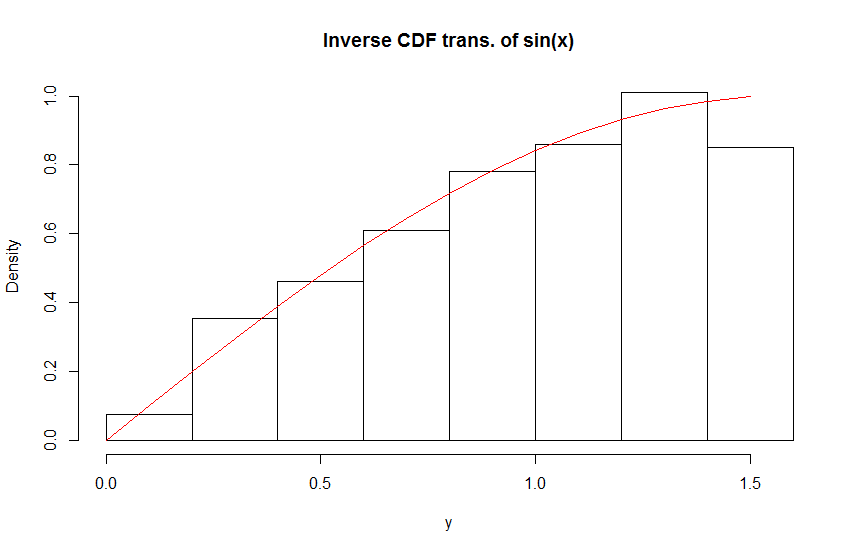
\includegraphics[width=\linewidth]{./figures/Rplot.png}
   	\end{subfigure}
\end{figure} 

The red line is the graph of $sin(x)$ from $(0, \pi/2)$. and the histogram is contains the samples from our inverse CDF, $arccos(x)$.

\subsection{Set up a rejection sampling method to sample from $p(x)$ using a proposal density $g(x)$. Plot the histogram and the true density for visual verification}
\textit{Hint: You can take $g(x)$ as the uniform density on the interval $(0,\pi / 2)$}. \\ \noindent\rule{2cm}{0.4pt} \\

\begin{lstlisting}[language=R]
arfunc = function(n=1000) {
  rv = rep(0,n)
  a = 0
  for(i in 1:n) {
    x = runif(1)
    if(x > -acos(x)) {
      rv[i] = x
      a = a + 1
    }
  }
  cat("Efficiency is ", a/n)  
  plot(rv)
  title("accept reject plot")
}
arfunc()
\end{lstlisting}

\begin{figure}[!htbp]
  	\centering
   	\begin{subfigure}[p]{0.8\linewidth}
    	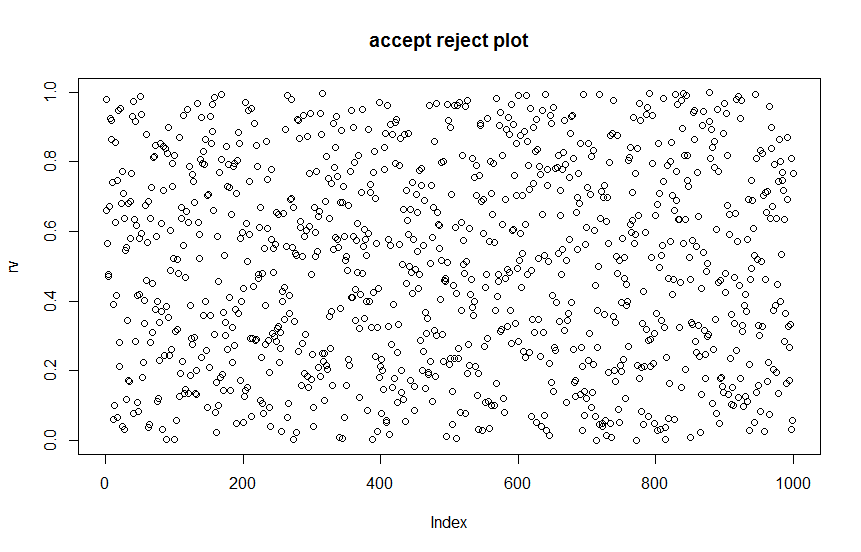
\includegraphics[width=\linewidth]{./figures/Rplot01.png}
   	\end{subfigure}
\end{figure} 

\section{Question 2}
Determine a method to draw samples from the distribution with PDF: $f(x) \propto exp(-x^{4} / 12)$, for $x \in \!R$.  Turn in derivation and code. Plot histogram and true density for visual verification. \\ \noindent\rule{2cm}{0.4pt} \\

We can relate this density to its general form, where $f(x) \propto exp(-kx^{n})$. In our case, $k=1/12$, and $n=4$.  Let $Y = X^{4}$. Note $x>0$ so $y>0$. We want to perform a change of variables so we can have our density in terms of $y$.  

$ \frac{dy}{dx} = 4x^{3}$. From the change of variables theorem, $f_y(y) = f_x(x) \mid \frac{dy}{dx} \mid$. Thus, $f_y(y) = exp(-x^{4}/12)\frac{1}{4}x^{-3}$.  Now we need to swap out $x$ for $y$.  Observe the relationship: $y=x^{4}$ Which is change to $x=y^{1/4}$. By subsitution, we have $$f_y(y)=exp(-y/12)\frac{1}{4}y^{-3/4}$$

Note that this is similar to the Gamma density: $$f(u) = \frac{\lambda^{\alpha}e^{-\lambda u}u^{\alpha - 1}}{\Gamma(\alpha)}, u \geq 0$$

However, we are sampling over all of $\!R$, so we need to do a coin-flip on every sample, and decide whether the sample must be negative or positive. 

\newpage
\begin{lstlisting}[language=R]
z = rgamma(1e5, shape = (1/4), rate = (1/12))
z = z^(1/4)
f = runif(1e5)
for(i in 1:1e5) {
  if(f[i] < 0.5) {
    z[i] = z[i] * -1
  }
}
hist(z, breaks = 30, freq = F, col = rgb(0.75,0.4,0.1,0.5)) # z is your sample
lambda = 1/12; alpha = 1/4
target <- function(x){exp(-lambda*x^(1/alpha))/
    integrate(function(x) exp(-lambda*x^(1/alpha)),0,Inf)$value}
curve(target,lwd=2,add=T)
\end{lstlisting}

\begin{figure}[!htbp]
  	\centering
   	\begin{subfigure}[p]{0.8\linewidth}
    	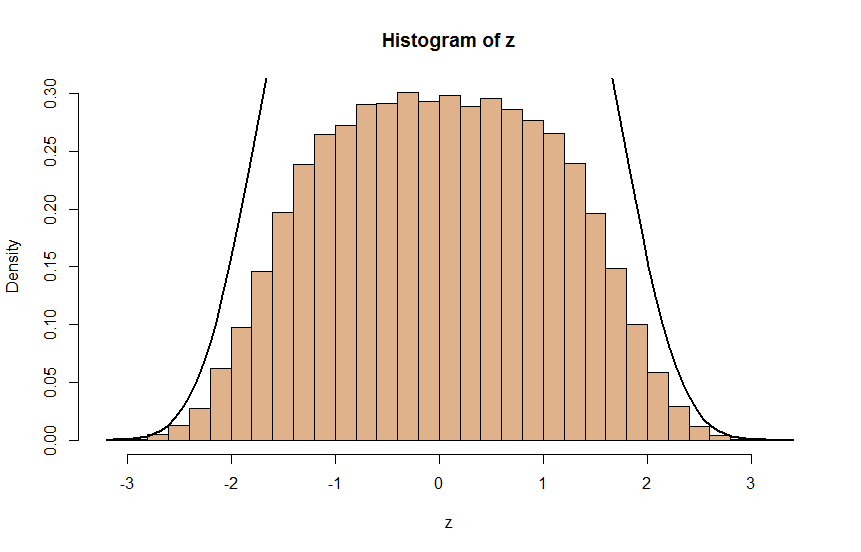
\includegraphics[width=\linewidth]{./figures/Rplot02.png}
   	\end{subfigure}
\end{figure} 


\section{Question 3}
Suppose that $X \in \!R^{nxn}$ is a random matrix with independent $\mathcal{N}(0,1)$ entries. Let $\ell_1$ be the smallest Eigenvalue of $S_n = X^{T}X/n$ and let $Y = n\ell_1$.  Edelman showed that as $n \rightarrow \infty$, the PDF of $Y$ approaches \\ 
{\Large $f(y) = \frac{1+\sqrt{y}}{2\sqrt{y}}e^{-(y/2 + \sqrt{y})}$, $0<y<\infty$ } 
\subsection{Develop a method to sample $Y$ from the density $f(y)$ given in the equation above. Show derivation and code. Plot histogram and true density for visual verification.}

\subsection{Test method by estimating $\!E(log(Y))$ by simple Monte Carlo, and giving a $99\%$ confidence interval. Edelman found that the answer was roughly -1.68788.}


\end{document}




